\chapter{Columnar Compression}
\label{columnar-compression}

Compression in column-oriented storage has been extensively researched \cite{abadi-col-comp, abadi-sparse-col, boncz-comp} in the world of \gls{rdbms}. The main idea of column-specific compression being, 1) the ability to compress each data column independently depending on its datatype and features like runs, sorted etc.; 2) high compression rates since adajcent elements in the column are similar; and 3) with some cases, ability to operate directly on compressed data. However, not all columnar compression techniques can be directly applied to the data-structures that we introduced in Chapter~\ref{c:columnar-storage}. In this chapter, we identify the set of requirements that we want to achieve by compressing our columnar structures. We then review existing compression techniques and propose a technique tha helps us fulfill our reuqirements.

We begin by exploring the set of requirements in Section~\ref{sec:col-existing}. Based on these requirements, we review the applicability of a number of existing columnar compression techniques. Section~\ref{sec:sparse} discusses the case of data sparsity in our columns and why existing solutions to compress spare columns are not applicable to our case. Finally, we end the chapter by introducing a new NULL compression algorithm, called \emph{prefixSum-based NULL compression}, that addresses the shortcomings of existing solutions to compress sparse columns, in Seciton~\ref{sec:prefixbased}.

\section{Directly Applicable Compressing Techniques}
\label{sec:col-existing}

We designed our columnar data structures for in-memory \gls{gdbms}. For these data structures, the focus with compression is not on achieving high compression ratios but to optimize for high decompression rates or to avoid decompression of data at all. There has been much research that studies compression techniques from the point of avoiding eager decompression of compressed data \cite{westmann-comp, dat-comp}. \cite{abadi-col-comp} abstracts out the high-level properties of a compression algorithm and use this information in query executor to operate directly on compressed data whenever possible. Our's is an identical requirement in the sense that operating directly on compressed data can avoid CPU overhead and increases the read throughput while reading from adjacency lists and property stores.

The design of vertex and edge property columns as described in sections \ref{sec:vertex-property-columns} and \ref{sec:edge-property-columns}, allows for random access of property values based on the positional offset in a column. Random lookups in a column can be performed intuitively once we decompress the entire column or a part of it. However, this involves the additional cost of decompressing elements that are not required to be read, thereby wasting CPU cycles. We can avoid this cost by randomly acessing elements from the compressed column, which is a step ahead of operating directly on the compressed data. Random accesses to a compressed column is possible only if the elements of column are encoded in \emph{fixed-bitwidth}, instead of variable-bitwidth. 

The only columnar compression techniques that keep the data in fixed-width bits are \emph{dictionary encoding} and \emph{bit-vector encoding}. Whereas, related techniques, \emph{Prefix Supression} and \emph{Frame of Reference (FOR)}, can be adopted to encode elements in fixed-bitwidth to make them appropriate for our case. For each of these techniques, we give a brief description of the technique and state its characteristics that makes it suitable for our use-case. We also give a high-level implementation of how a technique is used in our system.

\begin{itemize}
	\item \textbf{Dictionary encoding:} The dictionary encoding is perhaps the most common encoding scheme to be used in \gls{rdbms} and has also been adapted to the column stores \cite{abadi-col-comp, boncz-comp}. At a high-level. tt maps the values into more compact and shorter representations using a variety of schemes, like Huffmann encoding. Though a number of dictionary encoding schemes have been proposed \cite{boncz-comp, dat-comp, abadi-col-comp}, we use the one implemnted in \cite{abadi-col-comp} for the following reasons: 1) it encodes the elements in fixed-bitwidth, and 2) the packaging of multiple values together as a 32- or 64-bit word is space efficient and can be easily retrieved using dictionary.
	
	Specifically, in column with $n$ unique values, each value is encoded in fixed $l=log_2(b)$ bits. Each $p$ encoded elements (of width $l$) in a column are packed together using 1, 2, 3 or 4-byte word. For instance, if $l=3$, then $p=2$ can pack two elements in a 1 byte word, while for $p=5$, 5 elements can be packed in a 2-byte word, and so on. For decoding, a pre-populated map of possible words to its constituent elements is used to get the relevant constituent elements. The value of $p$ depends on the size of the map. 
	
	\item \textbf{Bit-vector encoding:} The bit-vector encoding scheme is used to encode columns with small number of unique elements. It encodes the column by having $n$ bit-strings, one for each unique element. A bit-string associated to the value has the bit set at postions where that value appears in the column. Accessing a random location $i$ in a column compressed by bit-vector involves inspecting the $i$th position of each bit-string till a set bit is found. Inspecting \emph{all} the bit-strings adds to the overhead which increases with the number of unique values in the column. Hence, encode a column using bit vectors only when the unique values are less than 50.
	
	\item \textbf{NULL Supression:} The idea of \texttt{NULL} suppression is to omit storing leading zero bits or prefix \texttt{NULL}s in a value \cite{beckmann:sparse}. Each value is, hence, encoded in a variable number of bits along with the count of bits used for storing the value. For an integer value 12, the number of bits in which it can be stored is 4, instead of default 32. We adopt this encoding to the columns with 2 modifications:
	\begin{enumerate}
		\item To make this encoding byte-aligned and easy to decompress, we store the values in variable bytes instead of in variable number of bits. Hence, an integer value can be encoded with either 1, 2, 3 or 4 bytes, with two extra bits needed to store the number of bytes. 
		\item We do not encode each element of the column separately in variable-bitwidth. Instead, the element is encoded in the number of bytes that is sufficient to encode the largest element in a column or a block in column. The number of bytes for encoding an element is, hence, given by $\lceil log_2(max_v+1)/8\rceil$, where $max_v$ is the maximum element in the column or block. The resultant column now has fixed-bitwidth elements and does not need to store an extra 2 bits for the number of bytes used.
	\end{enumerate}

	\item \textbf{Frame Of Reference(FOR): }This technique is similar to the previous, instead each element $e$ is stored as NULL supressed $e-b$, $b$ is called the \emph{base value} of the column or block. Generally, for an integer column, its smallest element is take as the base value. FOR is effective when the elements of column are clustered.
	
\end{itemize}

\section{Compressed Storage of Edge and Vertex ID Pairs in Adjacency Lists}
\label{sec:storage-optimizations}

In this section, we show how vertices and edges can be stored compactly in the adjacency lists using the new identification schemes that we introduced in Sections \ref{sec:vertex-property-columns} and \ref{sec:edge-property-columns}. Decomposing the IDs into multiple small components often enables us to factor out most of these components, when they are in the structure of the data.  
%either avoid storing components which are unnecessary or can be inferred, or store it in a compressed fashion using one of the compression techniques we describe in Chapter~\ref{columnar-compression}.

Recall that the ID of an edge $e$ in our new edge ID scheme contains 4 components: (i) edge label; (ii) source vertex ID; (iii) destination vertex ID; and (iv) positional offset of the properties of $e$ in property pages. Recall also that then ID of a vertex $v$ contains 2 components: (i) vertex label; and (ii) (label-level) positional offset. First, both the source or the destination vertex IDs can be omitted when storing an (edge ID, neighbor ID) pair because the source (destination) vertex ID is implied by the offset of the pair in the forward (backward) adjacency list and the destination (source) vertex ID is the neighbor ID, which is already stored in the pair. Second, we do not have to store the labels of the edges as in our storage of the adjacency lists, we store a different CSR-like structure for each edge label. Therefore the only parts that need to be stored are positional offsets for edge IDs, and vertex label and positional offsets of neighbor IDs. We next discuss further cases when the structure and multiplicities of edges allows us to factor some of these components out: \todo{I'm removing positional offsets being 1-2 bytes. That is basically trailing 0 compression (let's not call it null compression) and should appear under compression.}
%Finally, the positional offset can be stored cheaply as often they are not more than 1 or 2 bytes hence. This follows from the fact that the number of edges in most of the adjacency list is relatively small (by the power-law) and so are the number of elements in each page. 

%To sum up, each entry in the adjacency list stores a small (1-2 byte) positional offset and the neighbour vertex ID which itself comprises of vertex label and local positional offset. We now present some common scenarios that allow for even further compaction by choosing to omit to store certain components:

\begin{itemize}
	\item \textbf{Edge label determines a single neighbour vertex label.} In this very frequent case, an edge label is between pairs of nodes when the sources or destinations (or both) can have a single label . For instance, in our example graph, FOLLOWS edges are between vertices having label PERSON. In this case, we can factor out the vertex label component of neighbor ID.
		
	\item \textbf{Edges do not have properties:} This is also a frequently appearing case. That is the edges with a particular label do not have any structured or unstructured properties. In this case, notice that the edges do not need to be identifiable at all as the system will never access properties of these edges. Therefore, what distinguishes two edges are their neighbor IDs and edges with the same IDs are simply replicas of each other and are stored twice. Therefore, we can omit storing the positional offsets of edge IDs.
	
	\item \textbf{Single cardinality edges:} Recall from Section~\ref{} that the properties for single cardinality edges can be stored in vertex property columns. So by using the source or destination vertex IDs, we can directly read properties. Therefore, we can omit storing any positional offsets. 
		
\end{itemize}
All of the above case arise frequently in real world graph data. For example, in the LDBC benchmark dataset, X  out of Y many edge labels determine a single neighbour labels, X many do not have any properties, X many have single cardinality edges. This results in X many of them not requiring storing any neighbor vertex's labels or positional IDs, which implies that we only store a neighbor label-label positional offset, which can be stored with as few as 4 bytes. \todo{Fix.} 

% **** Let's not call NULL compression but "trailing 0 omission" and I think let's not talk about factoring things out 
%Using the new identification scheme and further applying the above-mentioned optimizations, the adjacent edges and neighbour vertices in adjacency lists by as less as a single piece of information. We can still further reduce the memory footprint of adjacency lists by applying compression on components of the edge that has to be stored after removing unnecessary ones. We use \emph{fixed-bitwidth NULL compression}, which we describe in Section~\ref{sec:col-existing}, to compress the components of edge in the adjacency lists. Using this technique, a particular component of each edge in an adjacency list is encoded as fixed-width elements by removing a common number of leading zero bytes (that will be determimined by the maximum element) from each of them. For example, if an adjacency list has edge $[e1, e2, e3, e4, e5]$ with the neighbour vertex labels $[1, 2, 1, 1, 2]$, then the neighbour vertex label is encoded in 1 byte in the adjacency list, instead of usual 4-byte INT. Similarly, if the same set of edges have neighbour's local positional offsets $[1000, 2000, 3000, 2, 1]$, then each offset is stored in 2 bytes in the adjacency list.

We show the decrease in memory footprint of the adjacency lists, with each optimization, over the LDB SnB dataset, with more than 1 billion edges, in Chapter~\ref{c:evaluation}. Our evaluations reveal that the new scheme with opportunities to perform immense compaction and compression can reduce the size of adjacency lists by upto 94x, storing barely over 6 bytes of data per indexed edge in the system.

\section{Columns with Sparse Data}
\label{sec:sparse}

Owing to the nature of property graph data, one can expect a large number of \texttt{NULL} values, even in the columns for structured properties. Hence, the compression scheme is required to avoid storing \texttt{NULL} values in the columns, in order to reduce memory footprint of sparse columns. Even with storing only the not-\texttt{NULL} elements in a column, it is desirable to access an element from the column randomly and in constant time without decompressing. 

A number of techniques has been proposed for dealing with \texttt{NULL} values in the column \cite{abadi-sparse-col}. One can treat \texttt{NULL}s in the column as another potential value in the domain of column's datatype which could then be compressed by any of the columnar compression scheme. For example, a column that is very sparse ($>95\%$ \texttt{NULL} values) can be effectively encoded using run-length encoding. Other compression techniques can also be used depending on the level of sparsity.

\begin{figure}
	\vspace{-20pt}
	\hfill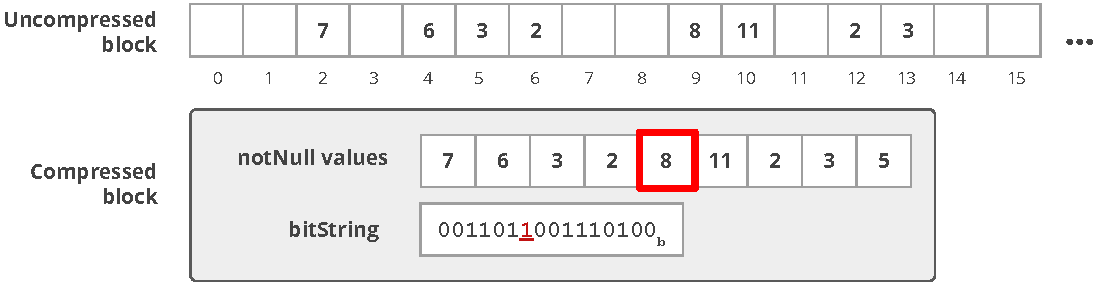
\includegraphics[scale=0.70]{img/null1}\hspace*{\fill}
	\captionsetup{justification=centering}
	\caption{\texttt{NULL} compression using bit-Strings.}
	\label{fig:null1}
	\vspace{-5pt}
\end{figure}

A more generalized \texttt{NULL} compression technique is based on using bit-string to indicate if the location is empty or not. In particular, we assign a \texttt{NULL} bit for each element in the column block to indicate if the value at that location is a \texttt{NULL} or not. Figure \ref{fig:null1} shows the \texttt{NULL} enocding of an uncompressed column using this scheme. The column is divided into block, where each compressed block holds 2 pieces of information: 1) a \textbf{non-\texttt{NULL}s array} that holds the non \texttt{NULL} values of the uncompressed block, and 2) a \textbf{bit-string} having a bit for each element in block, with 1's for non NULL elements. The storage overhead of the compressed block is only that of the bit-string which is 1 bit per element in the uncompressed block or 0.5 bit per non NULL element of the block that is 50\% occupied. Based on the sparsity, bit-string can be replaced by a list of offsets of non \texttt{NULL} elements in block for very sparse data, or list or ranges of non \texttt{NULL} elements for very dense data.

However, the above described compression scheme is not applicable to our scenario. Even though it is possible to operate on compressed column, the proposed scheme do not cater to our requirement of constant time random access. Reading from the compressed block involves iterating over the bit-string to calculate the location of the element in the non-\texttt{NULL}s array. For instance, in fig~\ref{fig:null1}, accessing the element at index 9 of uncompressed block involves counting the number of 1's till before index 9 in the bit-string, which is 4. Thus, the value is then read from index 4 of the non-\texttt{NULL} values array.

\section{PrefixSum-based NULL Compression}
\label{sec:prefixbased}

We present the solution to overcome the problem of constant time random reads in the existing solutions for compressing \texttt{NULL}s in sparse columns. The high-level idea is to do away with iteration over the bit-string while accessing the particular element in the compressed column.

\begin{figure}
	\vspace{-20pt}
	\hfill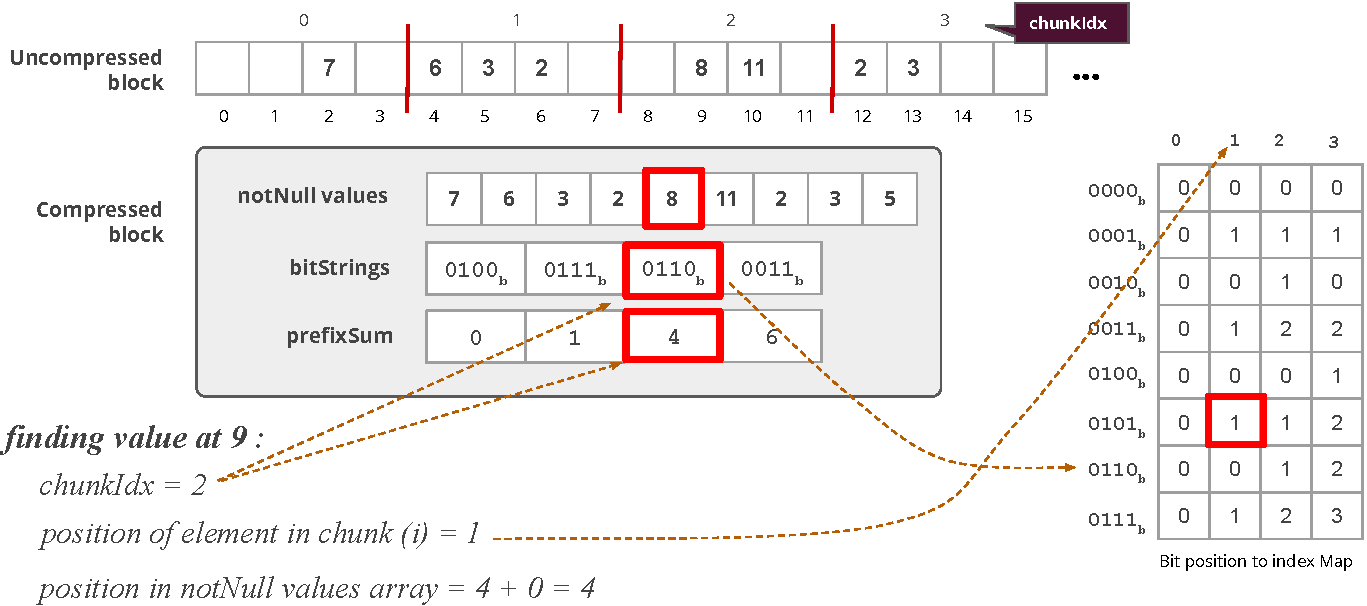
\includegraphics[scale=0.70]{img/null2}\hspace*{\fill}
	\captionsetup{justification=centering}
	\caption{PrefixSum-based \texttt{NULL} compression scheme. Chunk Size (n) = 4}
	\label{fig:null2}
	\vspace{-2pt}
\end{figure}

Figure~\ref{fig:null2} depicts compression of a sparse column using our scheme, which we call \emph{prefixSum-based NULL compression}. It divides a block into chunks of fixed size $n$. A compressed block contains 3 peices of information: 1) a non-\texttt{NULL}s array, 2) an array of bit-strings and, 3) an array of prefixSums. We store one bit-string of length $n$ and a prefixSum per chuck. Whereas the bit-string indicates positions in the chunk with non \texttt{NULL} elements, the prefixSum holds the number of non \texttt{NULL} elements in the uncompressed block before the current block. We also maintain a pre-populated static 2D map in the memory having size $(2^n, n)$. We call this \emph{bit-position-to-index map}. Let $b$ and $p$ respectively be the bit-string of length $n$ and prefixSum of a chunk. Given $b$ and the position $i$ in the bit-string, the bit-position-to-index map returns the number of 1's in $b$ uptil position $i$. Using the map, we can avoid iterating over the bit-string. We can directly to get the index of the element, at $i$ in the chunk, in the non-\texttt{NULL}s array. The index value returned by the map is relative to that chunk. This value, when added to $p$, gives the absolute index of the element, at $i$ in the chunk, in the non-\texttt{NULL} values array of the element.

\textbf{Dry run.} Suppose we need to find the element at index 9 of the uncompressed block. Given $n=4$, this element will appear in the 2nd chunk, say $c$, of the compressed block. The position $i$ of index 9 in $c$ is 1. Also, $c$'s bit-string and prefixSum are $\texttt{0110}_b$ and 4 respectively. The entry for ($\texttt{0110}_b$, 1) in the bit-position-to-index map is 0. Thus, the index of element at 9 in non-\texttt{NULL}s array is $4+0 = 4$.

The value of $n$ is chosen considering how big the bit index to position map do we want to fit in the memory. For $n = 16$, the size of the map comes out to be 1MB while that for $n=32$ is 128GB, which is impossible. Ideally, n can be upto 20, with the map size of 20MB. In our system, we use $n=16$. The overhead of bit-string and prefixSum can also be optimized. Since the bit-string takes a bit for each element in uncompressed block, the overhead depends on the size and number of prefixSums we have for an uncompressed block. If the size of prefixSum is $w$ and $n=16$, the overhead from prefixSums per element will be $w/16$ bytes. $w$ itself depends on the number of elements $N$ in the uncompressed block. For $n=2^16=32768$, $w=16$ and hence, the overhead of prefixSum is 1-bit per element.

Our NULL compression scheme can be used orthogonally with any of the applicable columnar compression techniques that we discussed in section~\ref{sec:col-existing}. We evaluate the effectiveness of our scheme in Chapter~\ref{c:evaluation} in effect to the storage savings by avoiding \texttt{NULL}s and the performance of queries when operating on \texttt{NULL} compressed columns.
















